\documentclass[10pt]{article}
\usepackage{itcep, stmaryrd, tikz, pgflibraryplotmarks, multicol, pgfplots}
\usepackage[margin=1in, nohead, pdftex]{geometry}

\topmargin -0.2in
\pagestyle{empty}
\singlespacing
\let\oldhat\hat
\renewcommand{\vec}[1]{\mathbf{#1}}
\renewcommand{\hat}[1]{\oldhat{\mathbf{#1}}}

\definecolor{light-gray}{gray}{0.95}
\newcommand{\code}[1]{\colorbox{light-gray}{\texttt{#1}}}

\newcommand{\headerclass}{Machine Learning Camp}
\newcommand{\headersection}{Day 2: Introduction to Classification}
\newcommand{\headertitle}{Going Bananas}

\def\C{\mathbb{C}}
\def\R{\mathbb{R}}
\parindent 0ex
\begin{document}
%==================================================================================================================================================
\headerclass\xspace \hspace{\stretch{1}} \headersection\\
\begin{center}{ \large \textbf{\headertitle} }\end{center}
%==================================================================================================================================================

Suppose we are trying to train a computer to recognize different types of fruits, based on their measurements. We've collected some data on the circumferences and heights of several apples, bananas, and pineapples, and we've plotted them in the chart below.

\begin{center}
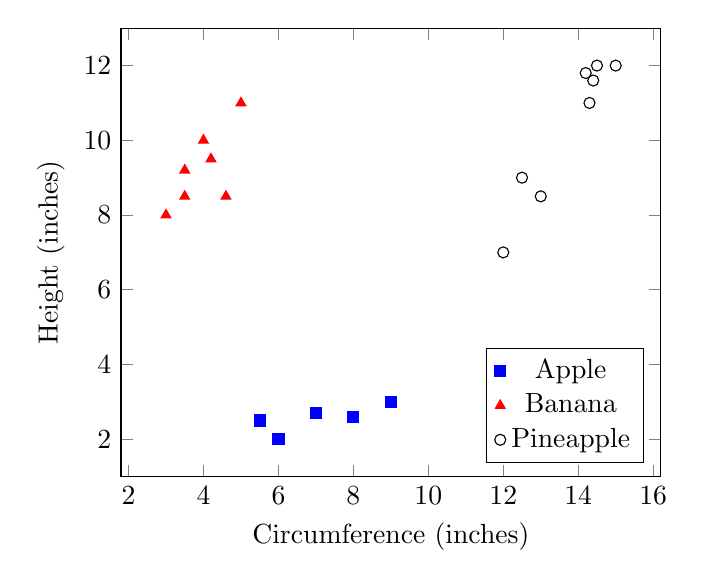
\begin{tikzpicture}
\begin{axis}[legend pos=south east,
    xlabel= {Circumference (inches)},
    ylabel= {Height (inches)},
  ]
    \addplot[
        scatter,only marks,scatter src=explicit symbolic,
        scatter/classes={
            a={mark=square*,blue},
            b={mark=triangle*,red},
            c={mark=o,draw=black,fill=black}
        }
    ]
    table[x=x,y=y,meta=label]{
        x    y    label
        15 12 c
        9 3 a
        4 10 b
        14.5 12 c
        14.3 11 c
        14.4 11.6 c
        14.2 11.8 c
        12 7 c
        13 8.5 c
        12.5 9 c
        6 2 a
        5.5 2.5 a
        8 2.6 a
        7 2.7 a
        5 11 b
        3 8 b
        3.5 8.5 b
        4.2 9.5 b
        3.5 9.2 b
        4.6 8.5
        
    };
    \legend{Apple,Banana,Pineapple}
\end{axis}
\end{tikzpicture}
\end{center}

\begin{enumerate}
\item If you have a fruit with circumference 13 inches and height 8 inches, would you expect it to be an apple, banana, or pineapple?
\vspace{1cm}

\item If you have a fruit with circumference 4 inches and height 7 inches, would you expect it to be an apple, banana, or pineapple?
\vspace{1cm}

\item If you have a fruit with circumference 8 inches and height 7 inches, would you expect it to be an apple, banana, or pineapple?
\vspace{1cm}

\item Given the circumference and height of a fruit, how do you decide if it's an apple, banana or pineapple? Does this method always work?
\vfill

\item Divide your graph into an apple region, a banana region, and a pineapple region. Can you do this in different ways? Compare your answers with a neighbor.

\end{enumerate}

\end{document}
